\documentclass[unnumsec,webpdf,contemporary,large,numbered]{oup-authoring-template}

\usepackage{amsmath,amssymb}
\usepackage{booktabs}
\usepackage{array}
\usepackage{tabularx}
\usepackage{graphicx}
\usepackage{url}
\usepackage{placeins}

\setlength{\textfloatsep}{10pt plus 2pt minus 2pt}
\setlength{\floatsep}{8pt plus 2pt minus 2pt}
\setlength{\intextsep}{8pt plus 2pt minus 2pt}

\graphicspath{{Fig/}}

\begin{document}

\journaltitle{Bioinformatics Advances}
\DOI{DOI added during production}
\copyrightyear{2026}
\pubyear{2026}
\vol{00}
\issue{0}
\access{Published: Date added during production}
\appnotes{Original Paper}
\firstpage{1}

\title[Evidence-guided LLM refinement]{DeepSeekCell: evidence-guided selective refinement for large language model annotation of single-cell RNA-seq}

\author[1]{Mohamed Kone}
\author[1,$\ast$]{Shulin Wang}
\author[1]{Gaoussou Haidara}

\address[1]{\orgname{School of Computer Science and Engineering, Hunan University}, \orgaddress{\city{Changsha}, \country{China}}}

\corresp[$\ast$]{Corresponding author. \href{mailto:books@hnu.edu.cn}{books@hnu.edu.cn}}

\received{Date}{0}{2026}
\revised{Date}{0}{2026}
\accepted{Date}{0}{2026}

\abstract{
\textbf{Motivation:} LLMs can interpret scRNA-seq marker genes, but indiscriminate second-pass inference is costly, difficult to audit and may spend computation on predictions that are already biologically consistent.\\
\textbf{Results:} We present DeepSeekCell, an evidence-guided marker-based annotation framework that maps first-pass LLM labels to the Cell Ontology, scores deterministic marker, ontology and tissue evidence, and selectively refines only conflicted clusters. In a paired six-dataset benchmark, all ablation arms reused the same cached first-pass response, enabling direct comparison of first-pass prompting, evidence scoring, confidence adjustment and selective refinement. Evidence-guided refinement increased mean macro-F1 from 0.733 to 0.794 and recovered 59.1\% of the corrections achieved by full refinement while refining only 6.4\% as many clusters, with 81.3\% correction efficiency versus 56.3\% for Random-k, 43.8\% for Confidence-k and 8.8\% for full refinement. Cross-model pilots with local Ollama models and an ontology-disabled ablation showed that the selector is not specific to DeepSeek and that marker/tissue evidence accounts for most of the selection signal, with ontology evidence providing an additional contribution. These results support evidence-guided selective refinement as a cost-aware and auditable strategy for allocating LLM reasoning in single-cell annotation.\\
\textbf{Availability and implementation:} DeepSeekCell is released under the MIT license at \url{https://github.com/mohkone/DeepSeekCell.git}. The archived software record is available at \url{https://doi.org/10.5281/zenodo.20680434}. The manuscript describes software version 0.1.0.\\
\textbf{Contact:} \href{mailto:books@hnu.edu.cn}{books@hnu.edu.cn}\\
\textbf{Supplementary information:} Supplementary tables and benchmark outputs are available with the source repository.
}

\keywords{single-cell RNA sequencing, cell type annotation, large language models, selective refinement, confidence calibration, Cell Ontology, DeepSeek, Ollama}
\keywords[Abbreviations]{ARI: adjusted Rand index; AURC: area under the risk--coverage curve; ECE: expected calibration error; LLM: large language model; NLL: negative log-likelihood; scRNA-seq: single-cell RNA sequencing}

\boxedtext{Key Messages}{
\begin{itemize}
\item DeepSeekCell treats second-pass LLM reasoning as a limited computational resource rather than a default step for every cluster.
\item A deterministic evidence selector recovered 59.1\% of full-refinement corrections while refining only 6.4\% as many clusters.
\item Evidence-k outperformed Random-k and Confidence-k under matched refinement budgets and generalized across DeepSeek and local Ollama models.
\end{itemize}}

\maketitle

\section{Introduction}

Single-cell RNA sequencing (scRNA-seq) enables high-resolution analysis of cellular heterogeneity across tissues, development and disease. A central interpretive step is assigning biological identities to transcriptionally defined clusters or individual cells. In practice, this process often relies on expert interpretation of marker genes, reference atlases and tissue context. Manual annotation is powerful, but it can be subjective, labor-intensive and difficult to reproduce across laboratories.

Automated annotation methods have improved scalability. Reference-based approaches such as SingleR and scmap compare query profiles with labeled references or projected cell states \cite{aran2019singler,singlerbook,kiselev2018scmap}. Marker- and model-guided approaches such as ScType, CellAssign, Garnett and CellTypist use curated marker combinations, probabilistic assignment, supervised classification or pretrained cell type models \cite{ianevski2022sctype,zhang2019cellassign,pliner2019garnett,dominguezconde2022celltypist}. These methods are widely useful, but they depend on the coverage, specificity and label granularity of reference data, marker databases or training sets.

Foundation models and LLMs have opened a complementary route for annotation. Single-cell foundation models such as scBERT, Geneformer, scGPT and scFoundation learn representations directly from expression data \cite{yang2022scbert,theodoris2023geneformer,cui2024scgpt,hao2024scfoundation}. General and biomedical LLMs have also been evaluated for gene set interpretation, biomedical reasoning and single-cell annotation \cite{hou2024gpt4,jin2024genegpt,luo2022biogpt,singhal2023medpalm,hu2025genesetllm,wang2025geneagent,xiao2025deepcellseek}. Recent systems including scExtract, AnnDictionary, CASSIA and consensus LLM approaches further show that language models can contribute to cell type annotation and biological interpretation \cite{wu2025scextract,crowley2025anndictionary,ye2025lict,xie2025cassia,yang2026mllmcelltype}. However, LLM annotations can be difficult to audit, may vary across models or prompts, and can be expensive if every uncertain prediction receives additional inference.

DeepSeekCell addresses this gap by reframing LLM-based cell type annotation as an evidence-allocation problem. Rather than simply mapping a first LLM answer to an ontology, the method scores deterministic biological evidence, detects conflict between marker support and model output, adjusts confidence, and selectively requests a second pass only for clusters where evidence suggests that additional reasoning is most likely to help. The workflow is shown in Fig.~\ref{fig:workflow}. The main contributions are summarized in Table~\ref{tab:features}: a marker-driven annotation framework, Cell Ontology normalization, evidence-adjusted confidence, selective self-refinement, compute-matched selector controls, native CellTypist comparison, and multi-model pilot experiments demonstrating that the selector is not specific to one LLM backend.

\begin{figure*}[!t]
\centering
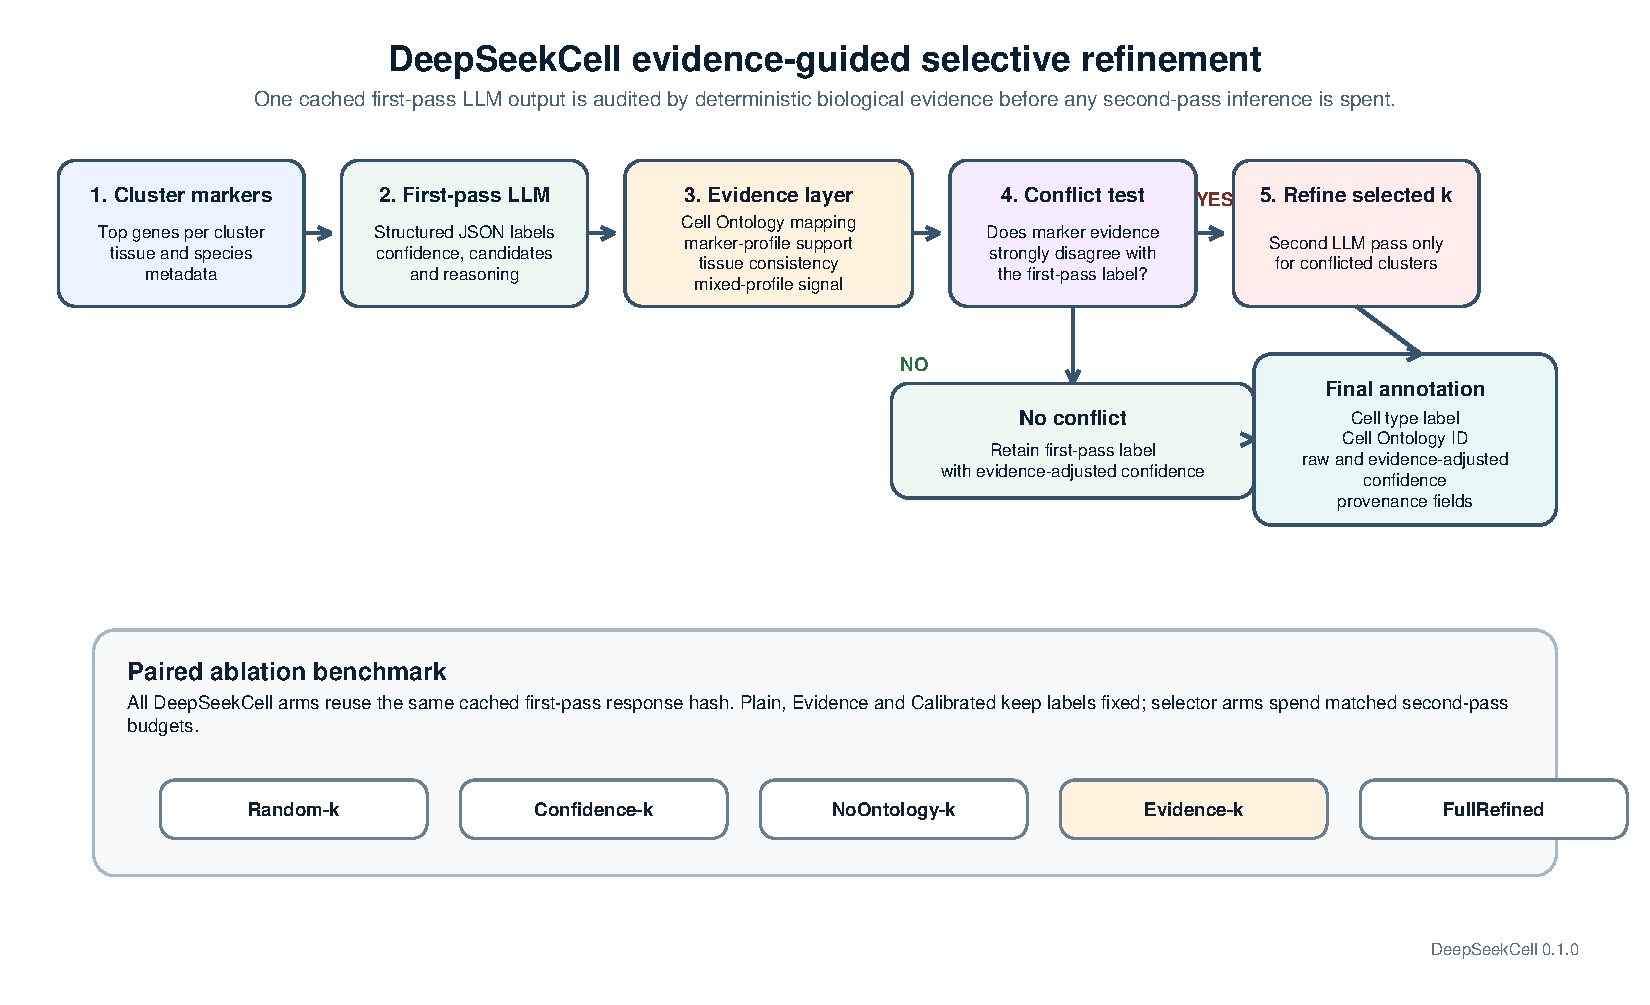
\includegraphics[width=\textwidth,height=0.68\textheight,keepaspectratio]{deepseekcell_workflow.pdf}
\caption{DeepSeekCell evidence-guided refinement algorithm. A cached first-pass LLM response is audited by deterministic marker, ontology and tissue evidence. Clusters without biological conflict retain the first-pass label with evidence-adjusted confidence, whereas conflicted clusters are routed to a selective second pass. The paired benchmark evaluates the proposed Evidence-k selector against Random-k, Confidence-k, NoOntology-k and FullRefined controls.}
\label{fig:workflow}
\end{figure*}

\begin{table*}[!t]
\caption{Main DeepSeekCell software and methodological features. The current manuscript evaluates version 0.1.0.}
\label{tab:features}
\centering
\begin{tabularx}{\textwidth}{p{0.29\textwidth}X}
\toprule
Feature & DeepSeekCell support\\
\midrule
Input representation & Cluster-level marker genes with optional tissue and species metadata\\
Model backends & DeepSeek API and local Ollama-compatible models\\
Ontology integration & Cell Ontology ID mapping, ontology label, match method and match score\\
Evidence scoring & Marker-profile support, ontology support, tissue consistency, marker--prediction consensus and mixed-profile penalty\\
Confidence output & Raw LLM confidence plus evidence-adjusted confidence\\
Selective refinement & Second LLM pass triggered only for evidence-conflicted clusters\\
Benchmark controls & Plain, Evidence, Calibrated, Random-k, Confidence-k, Evidence-k, NoOntology-k and FullRefined arms\\
External baselines & SingleR, ScType, scmap and native cell-level CellTypist where applicable\\
Interface & R functions and Shiny application with exportable reports\\
\bottomrule
\end{tabularx}
\end{table*}

\FloatBarrier

\section{Methods}

\subsection{Software architecture and annotation workflow}

DeepSeekCell is implemented as an R package with an interactive Shiny application. Marker processing standardizes gene symbols, removes duplicates and common low-information genes, and preserves the top marker genes selected from upstream clustering analysis. In the benchmark, the top 25 marker genes per cluster were used. The maintained model backends are the DeepSeek API and local Ollama models. DeepSeek was run with temperature 0 to reduce stochastic variation.

For each dataset or user submission, DeepSeekCell constructs a structured prompt containing tissue, species, cluster marker genes, output schema requirements and ontology-aware annotation instructions. The required schema includes cluster ID, predicted cell type, confidence, ranked candidate cell types, tissue consistency, mixed-cluster status and marker-based reasoning. The parser accepts valid JSON arrays as well as JSON embedded in code fences or short explanatory text.

Predicted labels are mapped to Cell Ontology terms using exact matching, synonym matching, tissue-context disambiguation, conservative fuzzy matching and fallback mappings for offline tests. The ontology loader uses the full Cell Ontology OBO file when available and caches parsed terms safely. The benchmark loaded 3,437 Cell Ontology terms from \texttt{data/cl.obo}.

\subsection{Evidence scoring and selective refinement}

The methodological core of DeepSeekCell is an evidence-guided selector that decides which first-pass annotations should receive a second reasoning pass. For cluster $i$, the first-pass annotation is augmented with raw LLM confidence $L_i$, ontology support $O_i$, marker support for the predicted label $M_i$, tissue-consistency support $T_i$ and marker--prediction consensus $S_i$. The displayed evidence-adjusted confidence is
\begin{equation}
C_i = m_i(0.35L_i + 0.25O_i + 0.25M_i + 0.10T_i + 0.05S_i),
\end{equation}
where $m_i=0.9$ for mixed or doublet-like clusters and $m_i=1$ otherwise. Scores are constrained to $[0,1]$. The weights were prespecified heuristic weights and frozen before the benchmark.

Marker evidence is calculated from tissue-specific and generic marker profiles. For cluster marker set $G_i$ and candidate cell type profile $P_c$, marker support is
\begin{equation}
M_{ic} = \frac{|G_i \cap P_c|}{\min(|P_c|, \max(3, |G_i|))}.
\end{equation}
The method records the strongest marker-supported cell type, marker support for the predicted cell type, the best competing marker support, matched markers and whether the evidence conflicts with the first-pass label. Ontology evidence measures semantic and nomenclatural support for the predicted label, whereas marker evidence provides a more independent biological consistency signal.

Selective refinement is triggered when deterministic evidence detects strong discordance between the first-pass label and a competing marker-supported identity. The refinement prompt contains the first-pass prediction, confidence, Cell Ontology mapping, strongest marker-supported identity, matched markers, conflict state, tissue and species metadata, and original reasoning. The model is instructed to retain the first-pass label unless stronger biological evidence supports revision. Every final annotation retains the first-pass label and confidence, flagging status, refinement status, label-change status and refinement reason.

\subsection{Benchmark datasets and baselines}

We evaluated DeepSeekCell under a closed-label, marker-driven cluster annotation scenario. This design matches the intended input representation: DeepSeekCell annotates cluster marker lists rather than raw expression matrices. Six datasets were included: PBMC, BaronPancreas, MuraroPancreas, TasicBrain, ZeiselBrain and ZilionisLung. Dataset characteristics are given in Table~\ref{tab:datasets}. Seurat-based preprocessing and clustering were used to produce marker lists \cite{hao2021seurat,seurat}. Three benchmark replicates used seeds 100, 200 and 300. Fixed datasets were deterministic across replicates, while ZilionisLung used seed-dependent cell subsampling.

\begin{table}[!t]
\caption{Benchmark datasets and preprocessing summary. Cluster counts are shown for the marker-based benchmark; ZilionisLung varied slightly across replicates because of seed-dependent subsampling.}
\label{tab:datasets}
\centering
\begin{tabular}{llllr}
\toprule
Dataset & Tissue & Species & Benchmark level & Clusters\\
\midrule
PBMC & PBMC & Human & Cluster markers & 8\\
BaronPancreas & Pancreas & Human & Cluster markers & 16\\
MuraroPancreas & Pancreas & Human & Cluster markers & 11\\
TasicBrain & Brain & Mouse & Cluster markers & 15\\
ZeiselBrain & Brain & Mouse & Cluster markers & 16\\
ZilionisLung & Lung & Human & Cluster markers & 16--18\\
\bottomrule
\end{tabular}
\end{table}

DeepSeekCell was compared with SingleR, ScType, scmap and CellTypist. SingleR, ScType and scmap predictions were converted to cluster-level labels by majority vote where needed. CellTypist was run in its native cell-level setting using tissue-aware pretrained models where available: an immune model for PBMC, an adult pancreatic islet model for pancreas and the Human Lung Atlas model for lung. Native cell-level CellTypist metrics were retained separately, and cluster-level CellTypist labels were derived by majority vote only for the shared cluster-level comparison. CellTypist was skipped for mouse brain datasets under the human-only baseline configuration.

\subsection{Paired ablation design}

The DeepSeek ablation benchmark used one cached first-pass response per dataset and replicate. The raw response text, prompt metadata and MD5 response hash were stored and reused across all DeepSeekCell arms, preventing API stochasticity from being interpreted as an algorithmic improvement. The evaluated arms are shown in Table~\ref{tab:ablation-arms}. Plain, Evidence and Calibrated intentionally use identical labels and therefore isolate confidence and evidence effects rather than classification effects.

\begin{table*}[!t]
\caption{DeepSeekCell ablation arms. Evidence-k is the proposed selector. Random-k, Confidence-k and NoOntology-k are compute-matched controls using the same per-dataset refinement budget as Evidence-k.}
\label{tab:ablation-arms}
\centering
\begin{tabularx}{\textwidth}{p{0.28\textwidth}ccccX}
\toprule
Arm & First pass & Evidence & Confidence changed & Second pass & Purpose\\
\midrule
DeepSeek-Plain & Yes & No & No & No & First-pass LLM baseline\\
DeepSeekCell-Evidence & Yes & Yes & No & No & Conflict detection without changing labels or confidence\\
DeepSeekCell-Calibrated & Yes & Yes & Yes & No & Uncertainty assessment without label changes\\
DeepSeekCell-RandomK & Yes & Yes & Yes & Selective & Compute-matched random selector\\
DeepSeekCell-ConfidenceK & Yes & Yes & Yes & Selective & Compute-matched low-confidence selector\\
DeepSeekCell-SelfRefined & Yes & Yes & Yes & Selective & Proposed evidence-guided selector\\
DeepSeekCell-NoOntologyK & Yes & Marker/tissue only & Yes & Selective & Ontology-disabled evidence selector\\
DeepSeekCell-FullRefined & Yes & Yes & Yes & Full & Approximate upper-bound refinement\\
\bottomrule
\end{tabularx}
\end{table*}

For the selector controls, $k$ was set to the number of clusters selected by Evidence-k within each dataset and replicate. Random-k refined $k$ randomly selected clusters. Confidence-k refined the $k$ lowest raw-confidence clusters. NoOntology-k used marker and tissue evidence while neutralizing ontology-derived evidence. FullRefined refined every cluster and served as an approximate upper bound.

\subsection{Evaluation metrics}

Annotation performance was evaluated using adjusted Rand index (ARI), macro-F1, exact cluster-level accuracy, balanced accuracy, ontology-aware clade accuracy, unknown-label rate, ontology coverage, runtime, token usage and estimated cost. Ontology-aware clade accuracy considers a prediction correct when predicted and reference labels are ontologically related at an accepted lineage level.

Refinement behavior was evaluated using the number of clusters flagged, number refined, wrong-to-correct revisions, correct-to-wrong revisions, unchanged errors and net correction rate. Correction efficiency was defined as wrong-to-correct revisions divided by the number of refined clusters. Recovery fraction was defined relative to the wrong-to-correct revisions achieved by FullRefined. Confidence quality was assessed using Brier score, binary correctness negative log-likelihood, expected calibration error, AUROC for distinguishing correct from incorrect predictions, area under the risk--coverage curve and reliability bins. Bootstrap confidence intervals for refinement-efficiency metrics were estimated by resampling dataset-replicate blocks.

\FloatBarrier

\section{Results}

\subsection{Overall annotation performance}

The final benchmark run completed 192 replicate-level result rows and 64 dataset-method summaries. DeepSeek ablation arms, ScType, SingleR and scmap were evaluated on all six datasets; CellTypist was evaluated on the four human datasets. Overall performance is shown in Table~\ref{tab:overall} and Figs.~\ref{fig:macroF1}--\ref{fig:accuracy}.

\begin{table}[!t]
\caption{Overall benchmark performance. Runtime is reported in seconds. CellTypist was evaluated on the four human datasets; the other methods were evaluated on all six datasets.}
\label{tab:overall}
\centering
\begin{tabular}{lrrrr}
\toprule
Method & Datasets & Macro-F1 & Accuracy & Clade accuracy\\
\midrule
DeepSeekCell-FullRefined & 6 & 0.808 & 0.810 & 0.862\\
DeepSeekCell-SelfRefined & 6 & 0.794 & 0.783 & 0.893\\
DeepSeek-Plain & 6 & 0.733 & 0.741 & 0.883\\
ScType & 6 & 0.749 & 0.773 & 0.778\\
SingleR & 6 & 0.466 & 0.479 & 0.757\\
scmap & 6 & 0.411 & 0.438 & 0.702\\
CellTypist & 4 & 0.558 & 0.612 & 0.656\\
\bottomrule
\end{tabular}
\end{table}

The first-pass DeepSeek annotation achieved mean macro-F1 of 0.733, exact accuracy of 0.741 and ontology-aware clade accuracy of 0.883. DeepSeekCell-SelfRefined increased mean macro-F1 to 0.794 and exact accuracy to 0.783 while maintaining high clade accuracy (0.893). FullRefined achieved the highest mean macro-F1 (0.808) and exact accuracy (0.810), but required refinement of every cluster.

\begin{figure*}[!t]
\centering
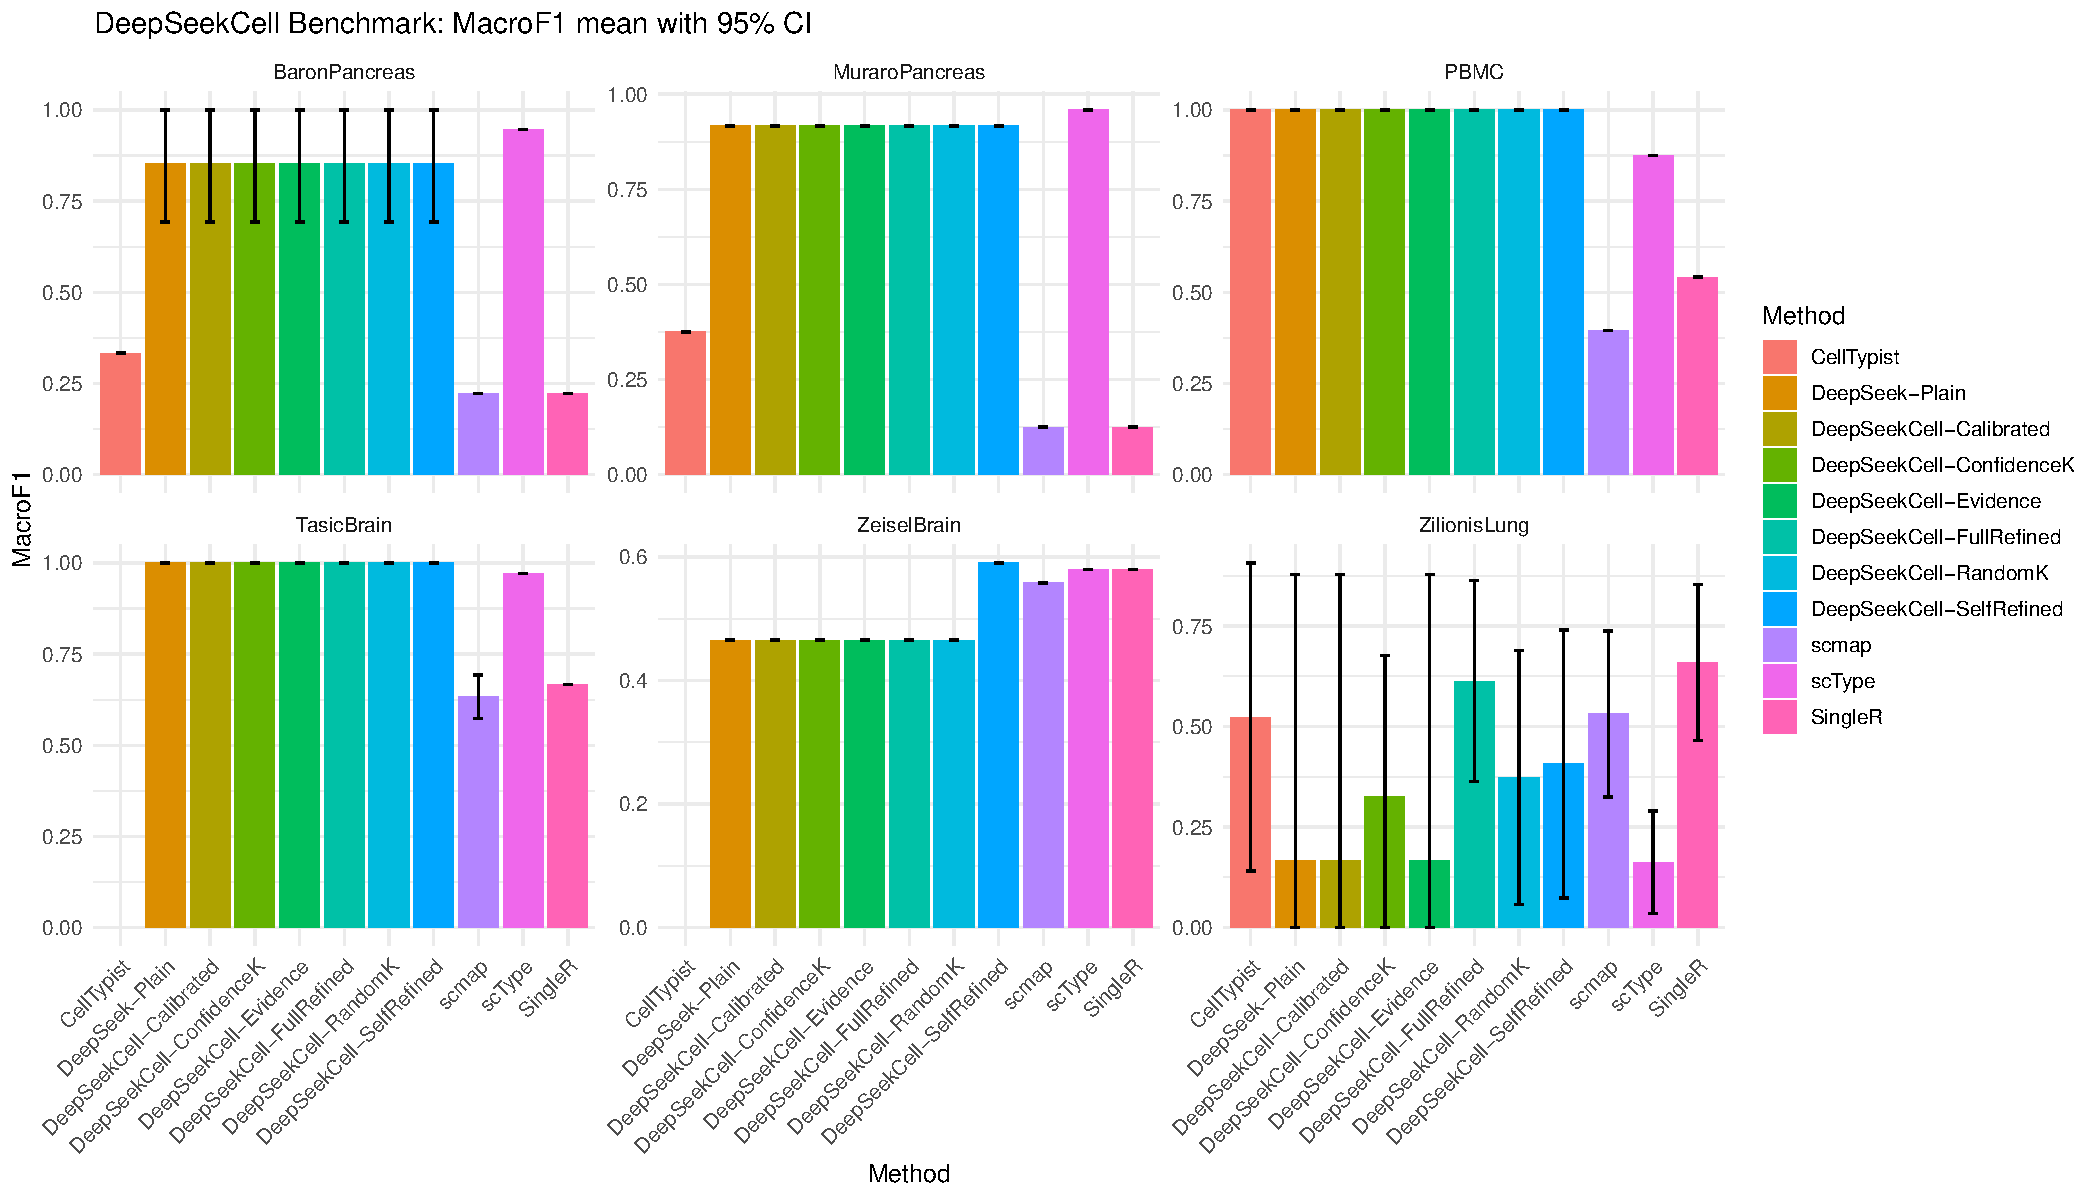
\includegraphics[width=\textwidth,height=0.68\textheight,keepaspectratio]{benchmark_macroF1.pdf}
\caption{Macro-F1 performance across benchmark datasets and methods. Bars represent the mean across three benchmark replicates. Error bars represent 95\% confidence intervals when replicate variability is present. CellTypist was evaluated on human datasets only.}
\label{fig:macroF1}
\end{figure*}

\begin{figure*}[!t]
\centering
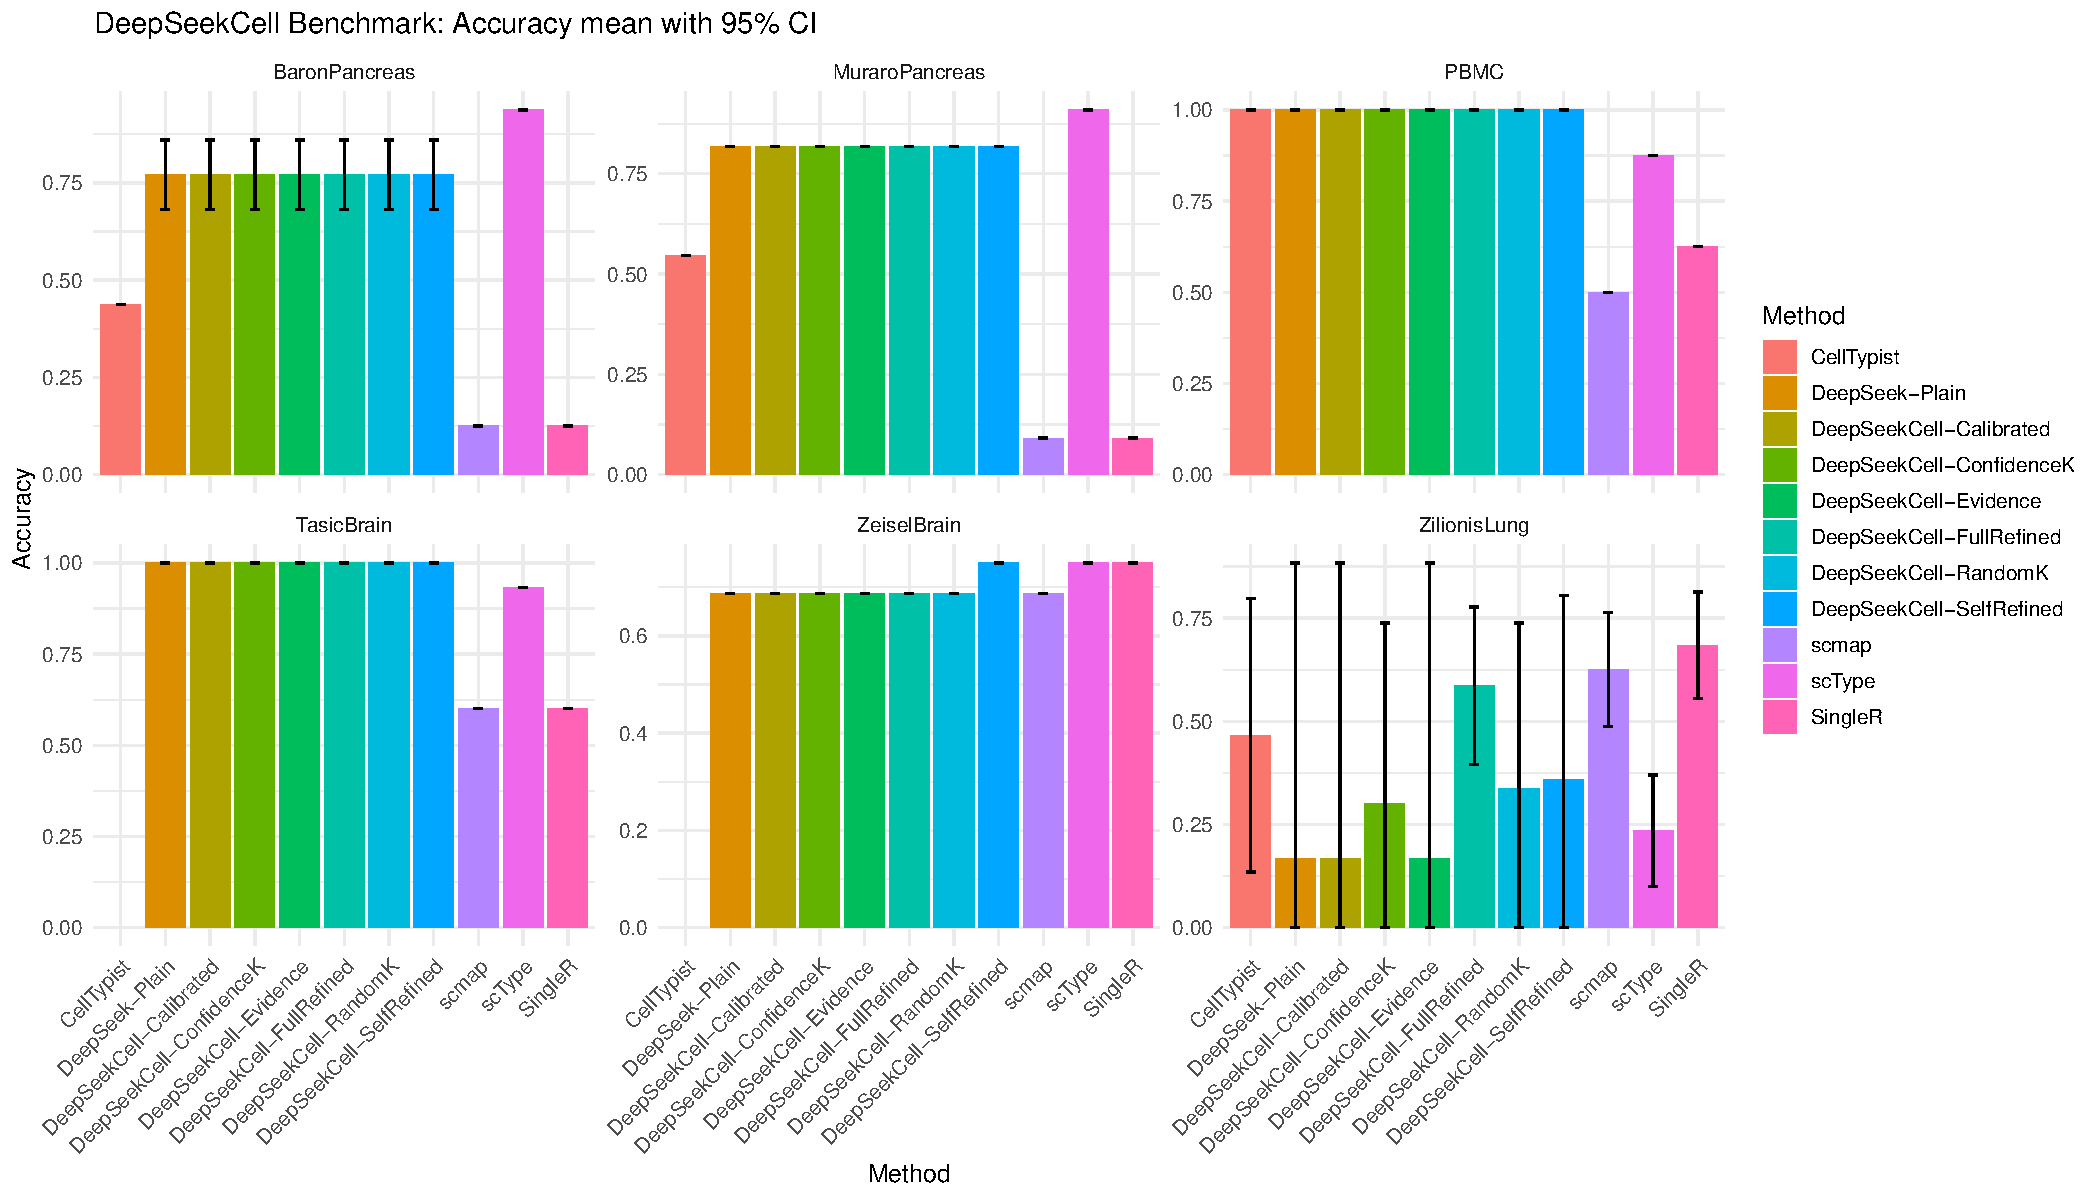
\includegraphics[width=\textwidth,height=0.68\textheight,keepaspectratio]{benchmark_accuracy.pdf}
\caption{Exact cluster-level annotation accuracy across benchmark datasets. DeepSeekCell-SelfRefined improved accuracy relative to the first-pass LLM while using selective second-pass refinement.}
\label{fig:accuracy}
\end{figure*}

\FloatBarrier

\subsection{Confidence calibration}

The evidence-adjusted confidence score improved average probability alignment. Brier score decreased from 0.139 for raw DeepSeek-Plain confidence to 0.127 for DeepSeekCell-Calibrated confidence, while binary correctness negative log-likelihood decreased from 0.449 to 0.418. Expected calibration error decreased from 0.138 to 0.105. After selective refinement, DeepSeekCell-SelfRefined obtained the lowest Brier score (0.125) and binary correctness negative log-likelihood (0.410) among the DeepSeekCell arms. AUROC decreased from 0.796 to 0.714 after calibration, indicating that the composite confidence improved average probability alignment but did not uniformly improve ranking of correct versus incorrect predictions.

\subsection{Controlled selective-refinement benchmark}

The central methodological experiment tested whether deterministic biological evidence can identify the clusters that benefit most from a second LLM pass. Results are shown in Table~\ref{tab:refinement-efficiency} and Fig.~\ref{fig:refinement-efficiency}. FullRefined corrected 22 initially wrong labels after refining 249 clusters, corresponding to 8.8\% correction efficiency. Evidence-guided selective refinement corrected 13 initially wrong labels after refining only 16 clusters, corresponding to 81.3\% correction efficiency. Under the same refinement budget of 16 clusters, Random-k corrected 9 labels and Confidence-k corrected 7 labels.

\begin{table}[!t]
\caption{Controlled refinement-selector efficiency. Correction efficiency is wrong-to-correct revisions divided by the number of refined clusters. Recovery fraction is calculated relative to the 22 wrong-to-correct revisions achieved by FullRefined.}
\label{tab:refinement-efficiency}
\centering
\begin{tabular}{lrrrr}
\toprule
Selector & Refined & Wrong-to-correct & Correct-to-wrong & Correction efficiency\\
\midrule
FullRefined & 249 & 22 & 0 & 0.088\\
Evidence-k & 16 & 13 & 0 & 0.813\\
Random-k & 16 & 9 & 0 & 0.563\\
Confidence-k & 16 & 7 & 0 & 0.438\\
\bottomrule
\end{tabular}
\end{table}

Evidence-guided selective refinement recovered 59.1\% of all corrections achieved by full refinement while refining only 6.4\% as many clusters. Its bootstrap 95\% confidence interval for correction efficiency was 71.4--100.0\%, compared with 0.0--85.7\% for Random-k, 0.0--58.1\% for Confidence-k and 0.0--20.8\% for FullRefined. No refinement strategy introduced incorrect revisions of previously correct annotations. Paired selector tests showed that Evidence-k significantly exceeded Confidence-k for wrong-to-correct revisions and net correction count after Benjamini--Hochberg correction (adjusted $P=0.039$ for both). Evidence-k also exceeded Random-k descriptively, although this difference was not significant in the current dataset-replicate sample.

\begin{figure*}[!t]
\centering
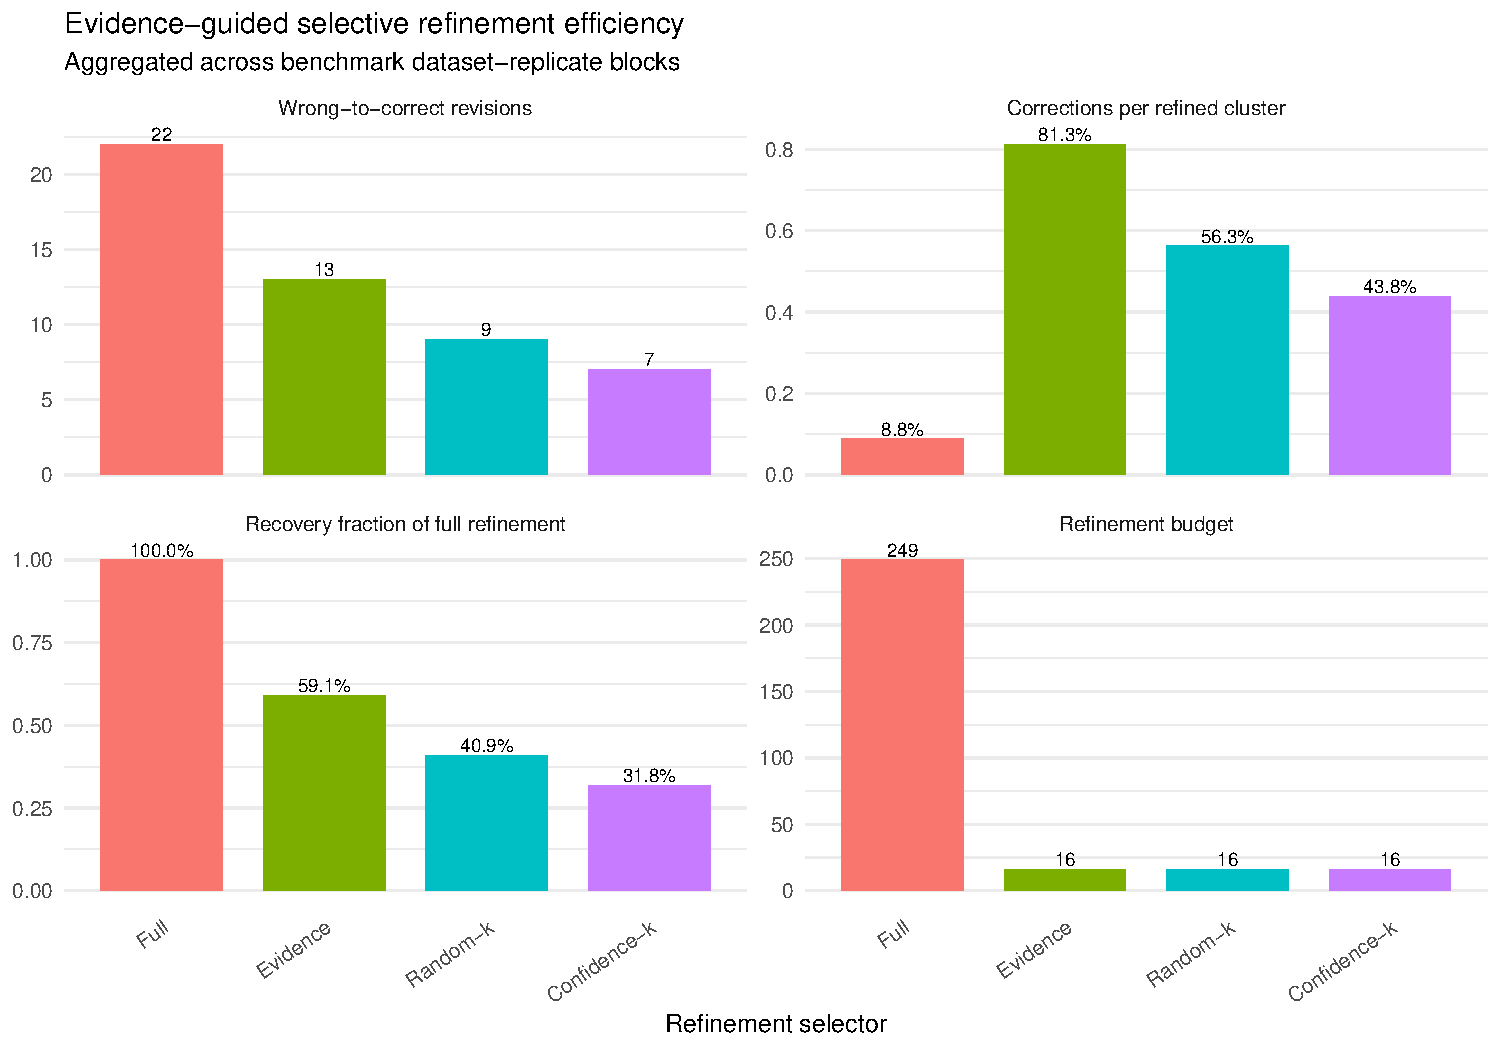
\includegraphics[width=\textwidth,height=0.68\textheight,keepaspectratio]{refinement_efficiency.pdf}
\caption{Evidence-guided selective refinement efficiency. Panels show wrong-to-correct revisions, correction efficiency, recovery fraction relative to full refinement and refinement budget. Evidence-guided selection recovered most of the attainable full-refinement corrections while using a small fixed refinement budget.}
\label{fig:refinement-efficiency}
\end{figure*}

\FloatBarrier

\subsection{Multi-model pilot and ontology-disabled ablation}

To test whether the selector was specific to DeepSeek, we ran the same selective-refinement protocol with local Ollama models. The multi-model pilot included ZilionisLung, PBMC and BaronPancreas for Llama 3.2 and Gemma2, and ZilionisLung for Mistral; unavailable local models were skipped explicitly. Across all informative model-dataset blocks, Evidence-k produced 26 wrong-to-correct revisions after 29 refinement calls (89.7\% correction efficiency), compared with 14/28 for Confidence-k (50.0\%) and 13/29 for Random-k (44.8\%). Evidence-k introduced no correct-to-wrong revisions. Selector efficiency and macro-F1 deltas are shown in Figs.~\ref{fig:multimodel-efficiency} and \ref{fig:multimodel-delta}.

\begin{figure*}[!t]
\centering
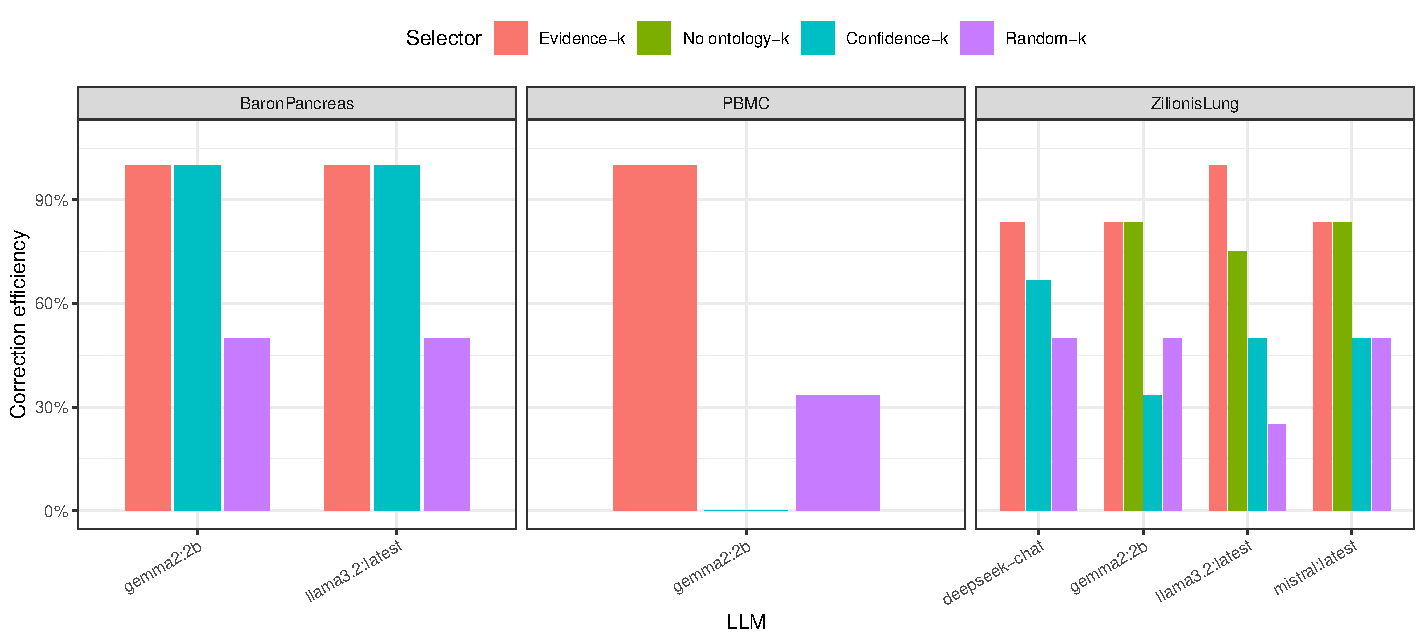
\includegraphics[width=\textwidth,height=0.68\textheight,keepaspectratio]{ollama_multimodel_all_selector_efficiency.pdf}
\caption{Selector correction efficiency in multi-model pilot experiments. Evidence-k consistently achieved the highest correction efficiency across DeepSeek-compatible and local Ollama settings, while local models incurred no API cost.}
\label{fig:multimodel-efficiency}
\end{figure*}

\begin{figure*}[!t]
\centering
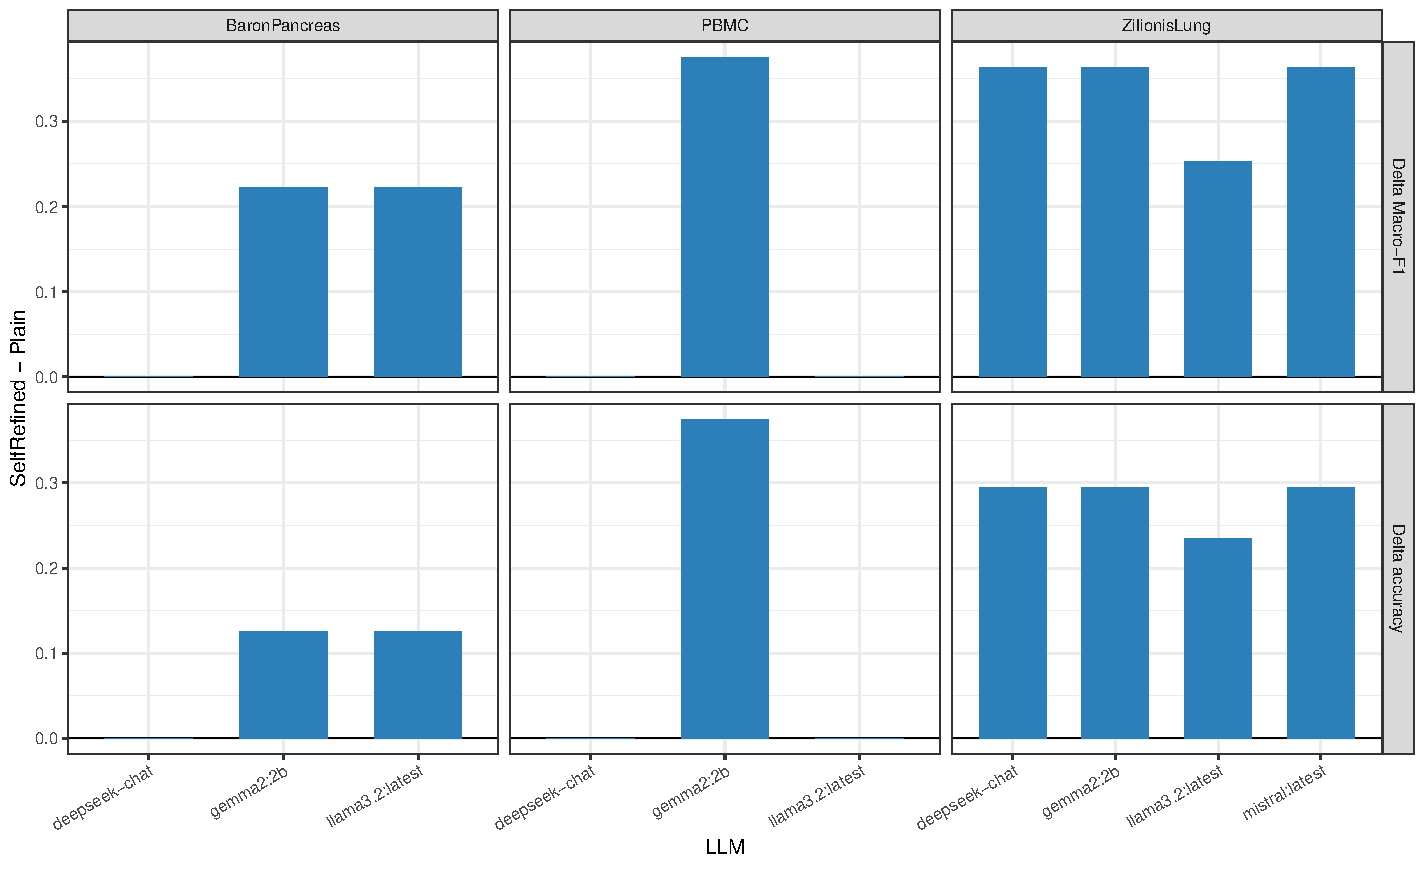
\includegraphics[width=\textwidth,height=0.68\textheight,keepaspectratio]{ollama_multimodel_all_plain_selfrefined_delta.pdf}
\caption{Macro-F1 changes from first-pass annotation to self-refined annotation in multi-model pilot experiments. Positive deltas indicate that selective evidence-guided refinement improved annotation performance relative to the same model's first-pass output.}
\label{fig:multimodel-delta}
\end{figure*}

We also evaluated an ontology-disabled selector in the ZilionisLung local-model pilot. NoOntology-k used marker and tissue evidence while neutralizing ontology evidence, with the same $k$ budget as Evidence-k. Results are shown in Table~\ref{tab:noontology}. NoOntology-k corrected 13 of 16 selected clusters (81.3\%), compared with 14 of 16 for Evidence-k (87.5\%) and 7 of 16 for both Confidence-k and Random-k. This result indicates that marker and tissue evidence account for most of the selector's benefit in this pilot, while ontology evidence provides a modest additional gain. The result should be interpreted as a targeted pilot rather than a full six-dataset confirmatory benchmark.

\begin{table}[!t]
\caption{ZilionisLung local-model ontology-disabled ablation. All selectors used the same per-model refinement budget as Evidence-k. Values are aggregated over Llama 3.2, Mistral and Gemma2.}
\label{tab:noontology}
\centering
\begin{tabular}{lrrr}
\toprule
Selector & Refined & Wrong-to-correct & Correction efficiency\\
\midrule
Evidence-k & 16 & 14 & 0.875\\
NoOntology-k & 16 & 13 & 0.813\\
Confidence-k & 16 & 7 & 0.438\\
Random-k & 16 & 7 & 0.438\\
\bottomrule
\end{tabular}
\end{table}

\FloatBarrier

\subsection{Dataset-level behavior and native CellTypist}

DeepSeekCell-SelfRefined achieved perfect macro-F1 in PBMC and TasicBrain. In pancreas datasets, ScType remained strongest (macro-F1 0.947 for BaronPancreas and 0.958 for MuraroPancreas), while DeepSeekCell-SelfRefined remained competitive (0.852 and 0.917). In ZeiselBrain, DeepSeekCell-SelfRefined achieved the highest macro-F1 (0.590), slightly above ScType (0.580) and SingleR (0.579), and improved over the first-pass LLM (0.465). In ZilionisLung, SingleR achieved the highest macro-F1 (0.659), while DeepSeekCell-SelfRefined improved substantially over the first-pass LLM (0.407 versus 0.166) using a limited refinement budget. Ontology-aware clade accuracy and runtime are shown in Figs.~\ref{fig:clade} and \ref{fig:runtime}.

CellTypist was evaluated in its native cell-level workflow on the four human datasets. Cell-level macro-F1 was 0.801 for PBMC, 0.298 for BaronPancreas, 0.362 for MuraroPancreas and 0.481 for ZilionisLung. For the shared cluster-level benchmark, cell-level CellTypist predictions were converted to cluster labels by majority vote, yielding cluster-level macro-F1 values of 1.000, 0.333, 0.375 and 0.524 for the same datasets. This native evaluation addresses CellTypist in its intended setting while retaining a secondary cluster-level comparison for consistency with the marker-based benchmark.

\begin{figure*}[!t]
\centering
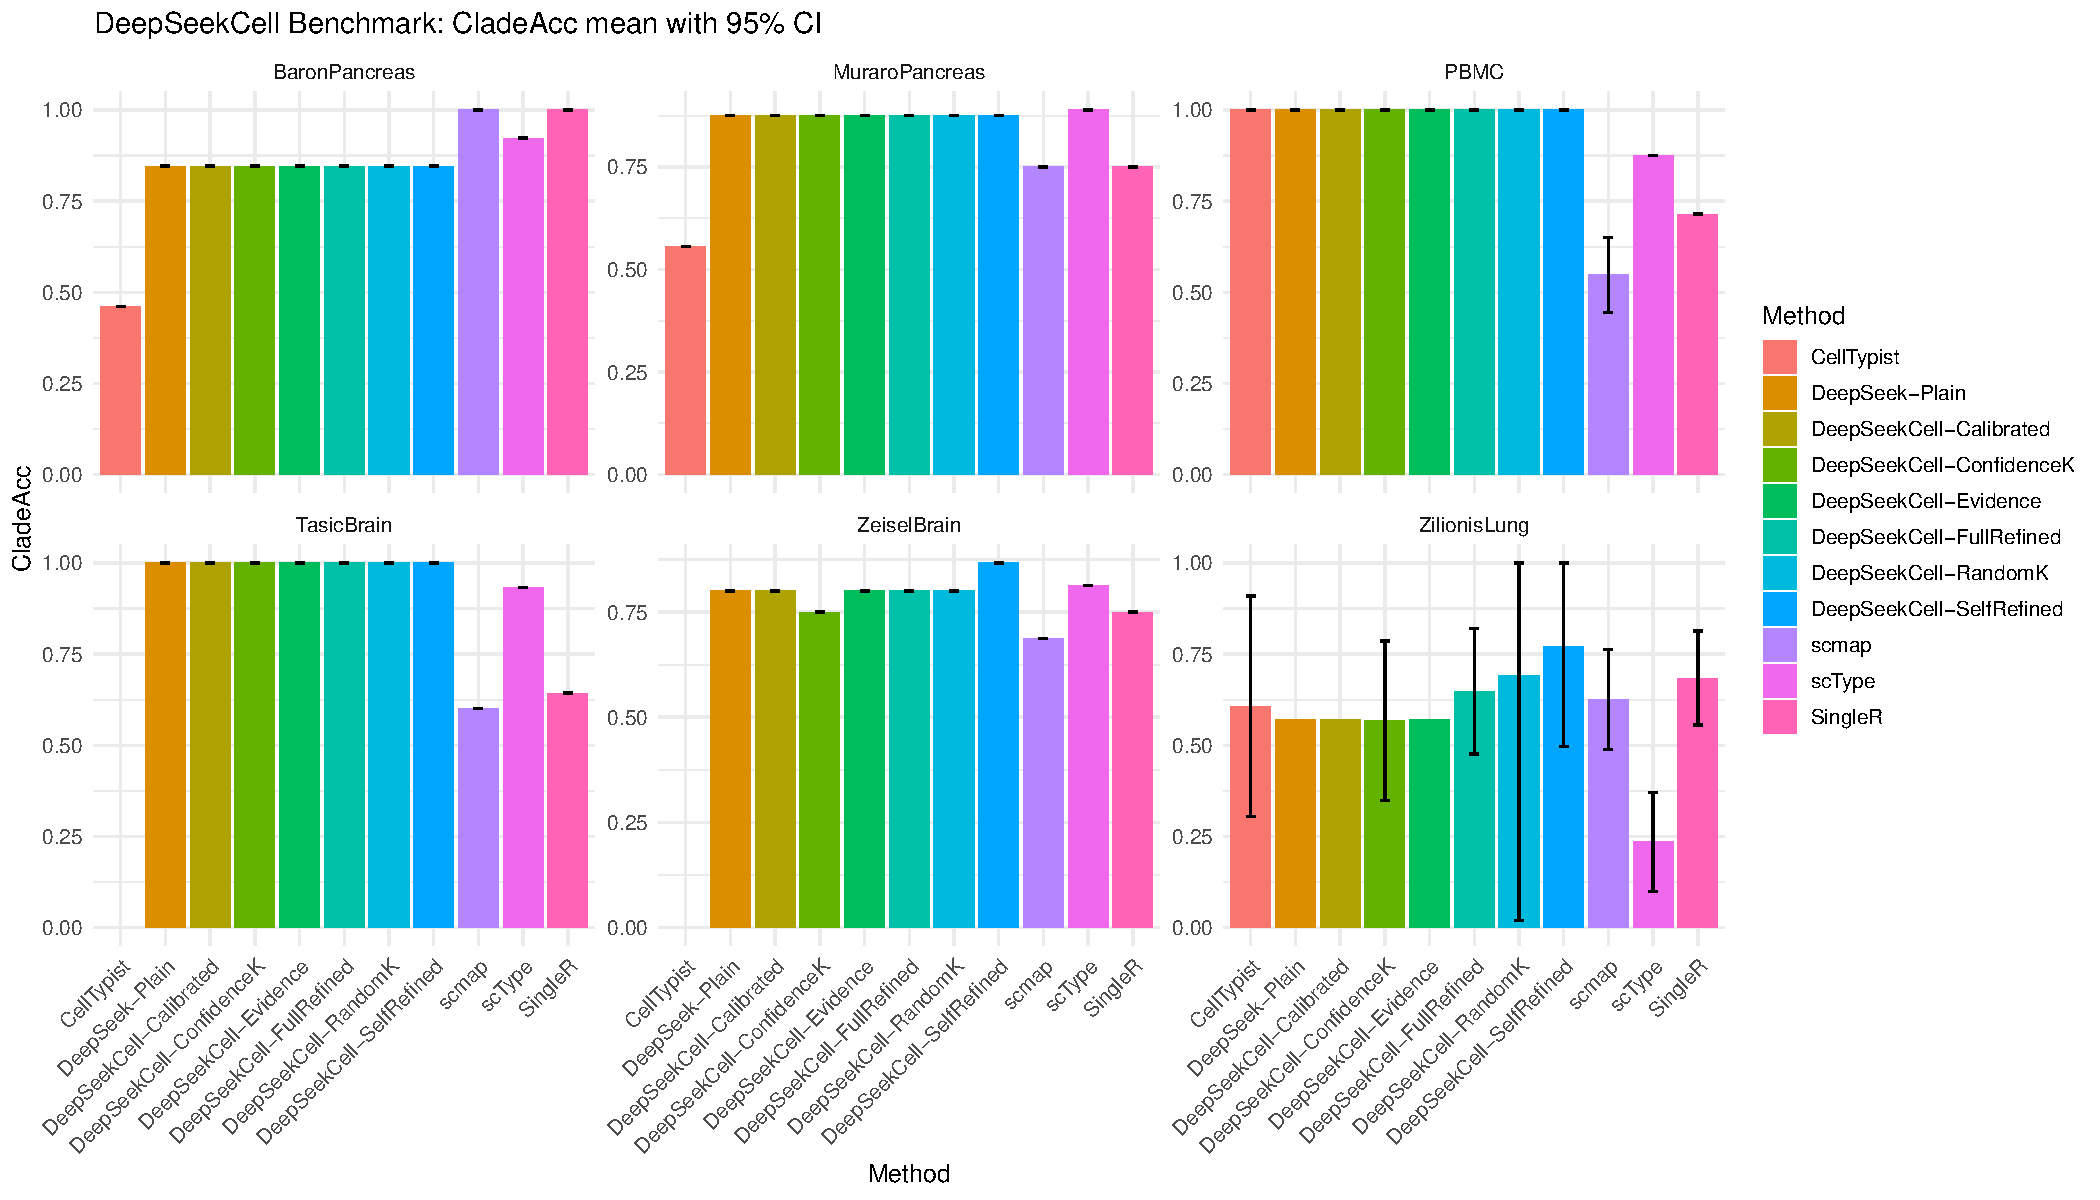
\includegraphics[width=\textwidth,height=0.68\textheight,keepaspectratio]{benchmark_clade_accuracy.pdf}
\caption{Ontology-aware clade accuracy across benchmark datasets. Clade accuracy gives partial credit when predicted and reference labels are ontologically related at an accepted lineage level.}
\label{fig:clade}
\end{figure*}

\begin{figure*}[!t]
\centering
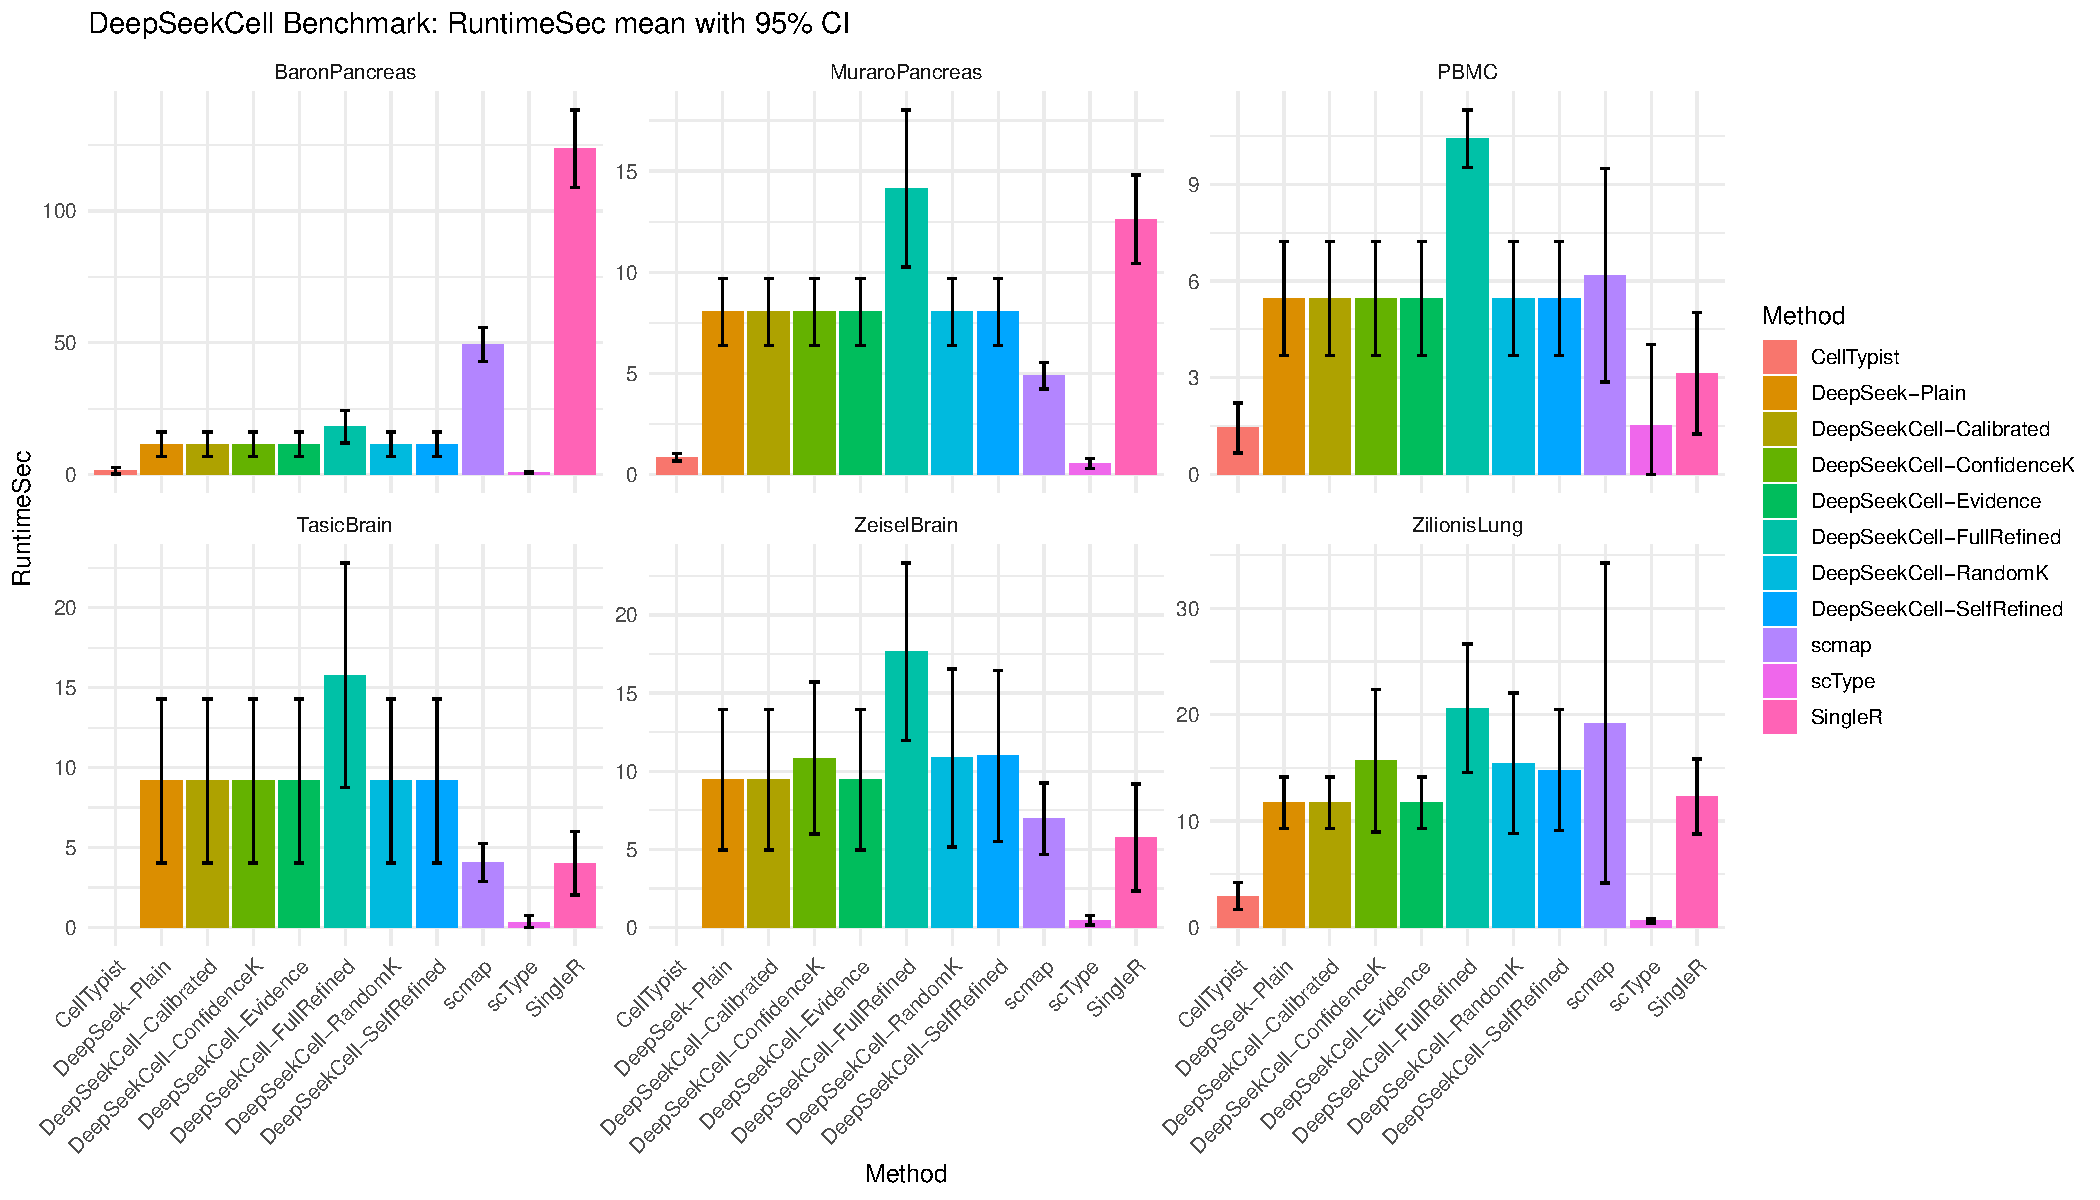
\includegraphics[width=\textwidth,height=0.68\textheight,keepaspectratio]{benchmark_runtime.pdf}
\caption{Runtime comparison across evaluated methods. DeepSeekCell-SelfRefined adds selective second-pass reasoning to the first-pass LLM, while FullRefined invokes a second pass for every cluster. ScType and CellTypist were fast baselines, while SingleR and scmap required longer runtime in several reference-based comparisons.}
\label{fig:runtime}
\end{figure*}

\FloatBarrier

\subsection{Computational efficiency and interface}

DeepSeek-Plain required a mean runtime of 9.22 seconds across the six datasets, while DeepSeekCell-SelfRefined required 9.99 seconds and FullRefined required 16.11 seconds. Across all dataset-replicate blocks, SelfRefined used 6,180 refinement tokens and 13.82 seconds of refinement runtime, compared with 75,385 refinement tokens and 124.13 seconds for FullRefined. Estimated refinement costs were USD 0.00110 for SelfRefined and USD 0.01353 for FullRefined. Thus, evidence-guided refinement recovered 59.1\% of the attainable corrections using 8.2\% of the full-refinement token budget and 11.1\% of the full-refinement runtime.

The Shiny application provides an interactive layer for entering marker genes, selecting tissue, species and model backend, running annotation, reviewing confidence and ontology fields, and exporting results (Fig.~\ref{fig:shiny}). The interface is a dissemination layer for the evidence-guided method rather than the main methodological contribution.

\begin{figure*}[!t]
\centering
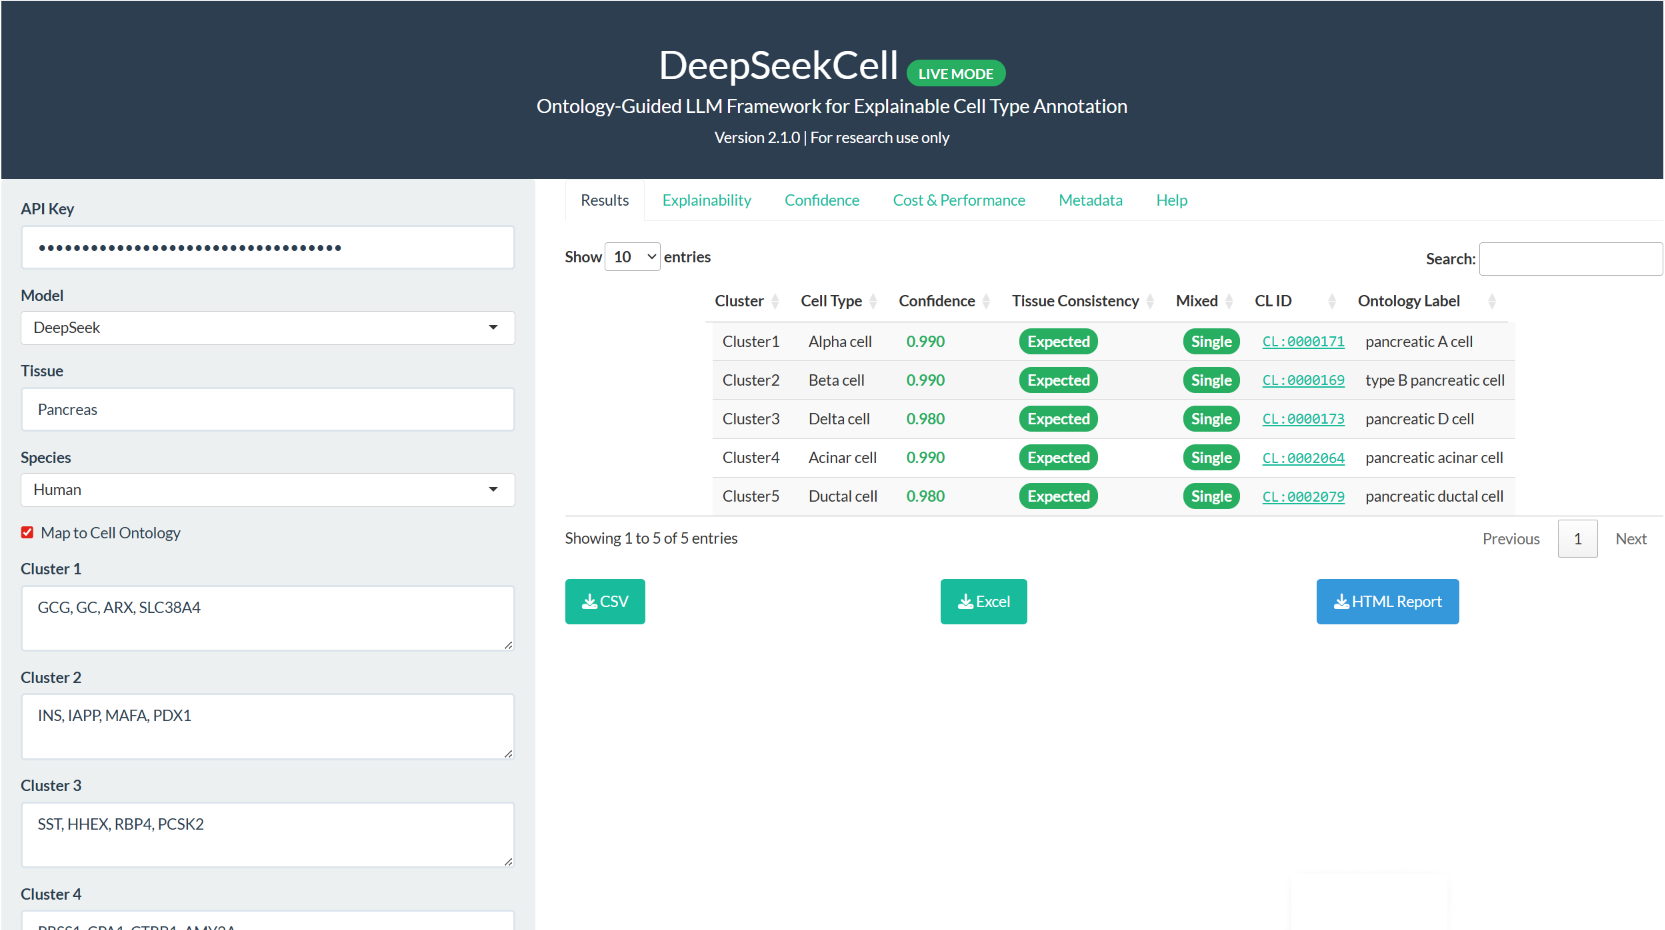
\includegraphics[width=\textwidth,height=0.68\textheight,keepaspectratio]{deepseekcell_shiny_interface.png}
\caption{DeepSeekCell Shiny interface for interactive cell type annotation. The application accepts cluster marker genes, displays predicted cell types with confidence scores and Cell Ontology identifiers, and provides explainability, validation, cost, metadata and report export views.}
\label{fig:shiny}
\end{figure*}

\FloatBarrier

\section{Discussion}

DeepSeekCell demonstrates that LLM-based cell type annotation can be improved by treating second-pass reasoning as a limited resource. The main contribution is not simply using DeepSeek for marker interpretation, but an evidence-guided selector that combines deterministic marker, ontology and tissue-consistency signals to identify clusters where additional reasoning is most likely to correct an error. This reframes annotation from a single prompting task into a cost-aware refinement problem.

Evidence-guided refinement is preferable to indiscriminate second-pass inference for both methodological and practical reasons. Methodologically, full refinement confounds error correction with extra model opportunity: any improvement could reflect repeated prompting rather than a better decision rule. Practically, full refinement spends tokens, time and API cost on many clusters whose first-pass labels are already supported by marker and ontology evidence, while also increasing the surface for unnecessary label changes. DeepSeekCell instead treats deterministic evidence as a triage layer. It preserves consistent first-pass annotations, routes only conflicted clusters to the second pass, and records why each cluster was or was not refined.

The fixed-budget selector experiment directly addresses an alternative explanation: that improvement arises merely because the LLM is asked a second time. Random-k, Confidence-k and Evidence-k received the same refinement budget, but Evidence-k corrected more initially wrong labels than either control and introduced no correct-to-wrong revisions. The multi-model pilot further supports model generality: the selector operates on structured first-pass outputs and deterministic biological evidence, and therefore can be paired with other instruction-following LLMs that return the required schema. The ontology-disabled ablation suggests that marker and tissue evidence provide most of the selection signal in ZilionisLung, with ontology evidence adding a smaller but measurable contribution.

The benchmark should be interpreted as a marker-driven cluster annotation benchmark rather than a raw expression matrix benchmark. This design matches the intended DeepSeekCell input representation and the common manual workflow in which analysts inspect top cluster markers before assigning identities. CellTypist was evaluated separately in its native cell-level workflow, while the cluster-level CellTypist comparison was included only for harmonized benchmarking.

This study has limitations. First, the benchmark is cluster-level and marker-guided for DeepSeekCell. Second, CellTypist comparisons were limited to human datasets under selected pretrained models. Third, the evidence weights were prespecified heuristics rather than learned calibration coefficients; future work should evaluate sensitivity analysis, held-out calibration and fitted calibration models. Fourth, ontology evidence is partly label-dependent: a wrong but valid label can still map well to the Cell Ontology, so ontology support should be interpreted as semantic support rather than proof of biological correctness. Fifth, marker profiles are manually curated and finite, so unsupported or poorly characterized cell states may receive conservative evidence scores. Sixth, the multi-model experiments are pilots and should be expanded across more datasets, model families and repeated runs. Finally, LLM-generated reasoning should be treated as an explanatory aid rather than independent biological proof.

\section{Conclusion}

DeepSeekCell introduces evidence-guided selective refinement for marker-based LLM annotation of scRNA-seq clusters. By combining structured first-pass annotation, Cell Ontology mapping, deterministic marker and tissue evidence, evidence-adjusted confidence and selective second-pass reasoning, the framework identifies a small subset of clusters where additional LLM inference is most useful. The benchmark shows that the selector recovers most attainable full-refinement corrections at a fraction of the refinement budget, supporting DeepSeekCell as a methods framework for explainable and cost-aware single-cell annotation.

\section{Conflict of interest}
The authors declare no competing interests.

\section{Funding}
The authors received no specific funding for this work.

\section{Data availability}
The source code is available at \url{https://github.com/mohkone/DeepSeekCell.git}. The archived GitHub-Zenodo software record is available at \url{https://doi.org/10.5281/zenodo.20680434}, with all-version concept DOI \url{https://doi.org/10.5281/zenodo.20680433}. Benchmark scripts are provided in the repository benchmarks directory, and the README documents a fresh-clone reproduction workflow, including reuse of cached LLM responses through the \path{DEEPSEEKCELL_USE_LLM_CACHE=true} setting. Benchmark outputs include the full and summary result tables, ablation confidence-quality metrics, refinement-behavior summaries, refinement-efficiency summaries, selector Wilcoxon tests, native CellTypist metrics and multi-model pilot summaries. Large external resources, including the full Cell Ontology OBO file and ScType database, should be obtained according to their upstream licenses.

\section{Author contributions}
M.K., S.W. and G.H. conceived the study, developed the DeepSeekCell software and Shiny platform, designed and interpreted the benchmark analyses, and wrote and revised the manuscript. All authors reviewed and approved the final manuscript.

\section{Acknowledgements}
The authors thank the developers and maintainers of the open-source single-cell and ontology resources used in this study.

\bibliographystyle{oup-plain}
\bibliography{deepseekcell_bioinformatics_advances_refs}

\end{document}
